%
% oberflaeche.tex
%
% (c) 2021 Prof Dr Andreas Müller, OST Ostschweizer Fachhochschule
%
\documentclass[tikz]{standalone}
\usepackage{times}
\usepackage{amsmath}
\usepackage{txfonts}
\usepackage[utf8]{inputenc}
\usepackage{graphics}
\usetikzlibrary{arrows,intersections,math}
\usepackage{ifthen}
\begin{document}

\newboolean{showgrid}
\setboolean{showgrid}{false}
\def\breite{7}
\def\hoehe{4}

\begin{tikzpicture}[>=latex,thick]

% Povray Bild
\node at (0,0) {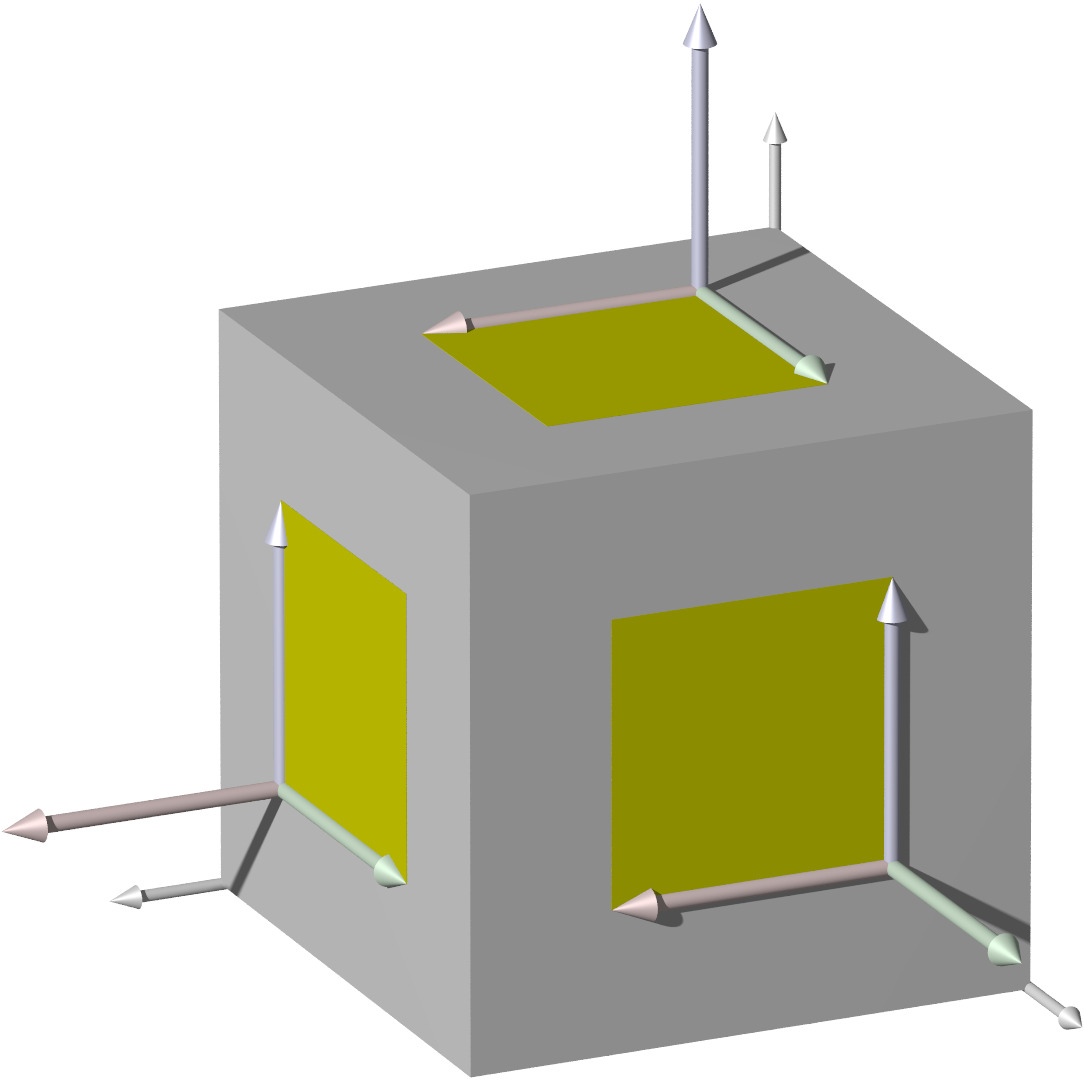
\includegraphics[width=8.6cm]{oberflaeche.jpg}};

% Gitter
\ifthenelse{\boolean{showgrid}}{
\draw[step=0.1,line width=0.1pt] (-\breite,-\hoehe) grid (\breite, \hoehe);
\draw[step=0.5,line width=0.4pt] (-\breite,-\hoehe) grid (\breite, \hoehe);
\draw                            (-\breite,-\hoehe) grid (\breite, \hoehe);
\fill (0,0) circle[radius=0.05];
}{}

\node at (-3.6,-2.85) {$x^1$};
\node at (4.5,-3.9) {$x^2$};
\node at (2.1,3.5) {$x^3$};

\node at (0.3,2.15) {$\vec{e}_1$};
\node at (1.85,1.95) {$\vec{e}_2$};
\node at (1.0,3.3) {$\vec{e}_3$};
\node at (0.7,1.5) {$\vec{e}_1\wedge\vec{e}_2$};

\node at (1.8,-3.05) {$\vec{e}_1$};
\node at (3.1,-1.4) {$\vec{e}_3$};
\node at (3.3,-3.3) {$\vec{e}_2$};
\node at (1.8,-1.6) {$\vec{e}_3\wedge\vec{e}_1$};

\node at (-2.4,-0.5) {$\vec{e}_3$};
\node at (-3.5,-1.9) {$\vec{e}_1$};
\node at (-1.5,-2.7) {$\vec{e}_2$};
\node at (-1.4,-1.3) {$\vec{e}_2\wedge\vec{e}_3$};

\end{tikzpicture}

\end{document}

